The Machine Learning software used was the WEKA software through the R language because it was applicable for the problem in hand. Almost all of WEKA's classifiers were used, with the \textit{default} paramters, including: \textbf{BayesNet, BFTree, ConjunctiveRule, DecisionTable, FT, HyperPipes, IBk, J48, J48graft, JRip} and others \cite{ml:csd}.
\\\\
To train the classifier on the problem instances the first step was modeling the instances. This step aims to convert a given problem instance into a data instance that is applicable to the classifier to train on. In our case the problems instances are CSP instances with the alldiff constraint, the CSP problem can represented as a set of constraints and these constraints can be modeled as a graph $G=(V,E)$ where the vertices in that graph represents the decision variables of the CSP along with their domains, and the edges are the constraints. For example, there will be an edge between vertix $V_{1}$ and vertix $V_{2}$ if and only if there is a constraint that bounds the two vertices together, Such a graph is called, The Constraint Network. To illustrate Figure \ref{cs:nw} shows the Constraint Network for a CSP problem instance:
\begin{figure}[h!]
  \vspace{1 cm}
  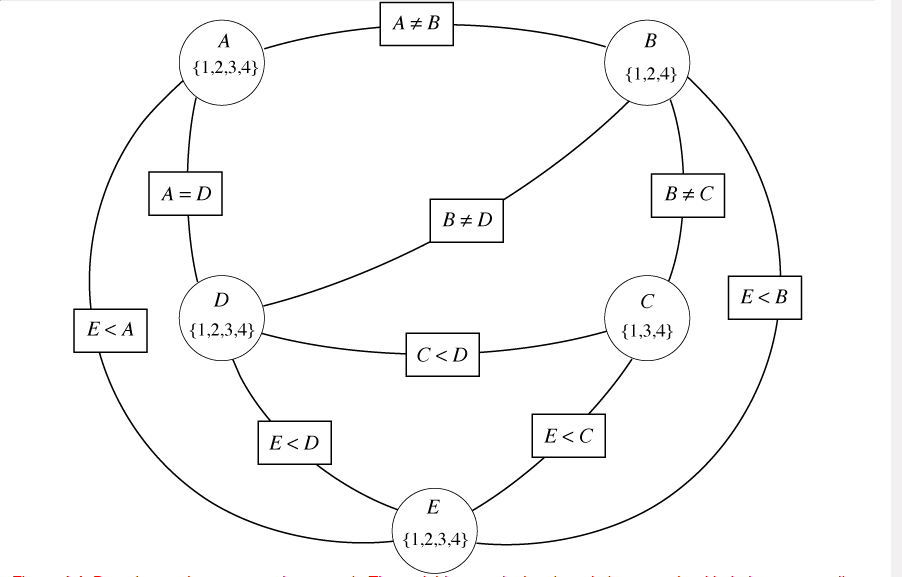
\includegraphics[width=1.0\textwidth]{images/constraint_nw.png}
  \caption[ ]{the Constraint Network for a CSP problem instance}
  \label{cs:nw}
\end{figure}

After converting the CSP into a Constraint Network a set of attributes is calculated. These attributes are to measure important features in the Constraint Network for the instance. Some of the attributes are:
\begin{itemize}
  \item \textbf{Edge density:} The number of edges in G divided by the number of pairs of distinct vertices.\\
  \item \textbf{Clustering coefficient For a vertex $v$ : } the set of neighbours of $v$ is $n(v)$. The edge density among the vertices $n(v)$ is calculated. The clustering coefficient is the mean average of this local edge density for all v \cite{f:feat}.\\
  \item \textbf{Normalised degree:} The normalised degree of a vertex is its degree divided by $|V|$. The minimum, maximum, mean and median normalised degree are used.\\
  \item \textbf{Variable domains:} The quartiles and the mean value over the domains of all
  variables.\\
  \item \textbf{Constraint arity:} The quartiles and the mean of the arity of all constraints
  (the number of variables constrained by it), normalised by the number of
  constraints.\\
\end{itemize}

These attributes along with others \cite{ml:csd} are calculated as numerical values. The numerical values are then applied to the classifier as a training data instance. The goal was to create a large set of the attributes to cover as much of the important factors as possibles. The more important the factor is the more that it affects the performance of different implementations \cite{ml:csd}. However, computing this large set of attributes required a significant amount of time that can usually reach a penalty of 27s per instance. And that time is added to the penalty of the solver itself which on average was only 0.2s per instance. And so, this makes the classifier slower than the default implementation \cite{ml:csd}. After considering this problem, The number of computed features was reduced and this lead to a significant improvement with an average of 5s per instance. Figure \ref{perf:speedup} shows the speedup achieved by the meta-classifier after computing the cheap set of features instead of computing all of them.
\\
\begin{figure}[h!]
  \vspace{1 cm}
  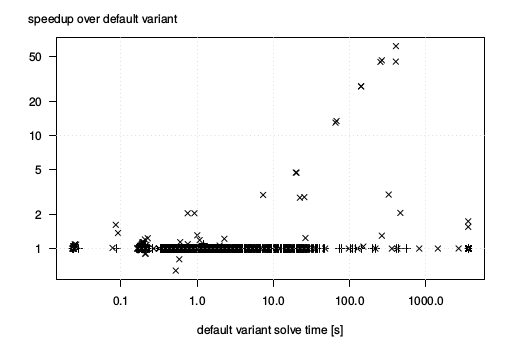
\includegraphics[width=1.0\textwidth]{images/speedup.png}
  \caption[ ]{Speedup achieved by the meta-classifier using the set of cheaply-computable
features.}
  \label{perf:speedup}
\end{figure}

The classifier was trained on 277 benchmark instances from 14 different problem classes chosen to include as many instances as possible. However, there was an important observation and that is due to the variety of the problem classes the classifier could be trained wrongly on them. But the goal here was not to train the classifier on as many different classes as possible, instead the goal was to classify the important problem classes correctly. So, in order to overcome this problem it was decided to ignore the classic Machine Learning performance measures. Measuring the performance was done in terms of the misclassification penalty, which as defined in \cite{ml:csd}, is the additional amount of CPU time required by the classifier when not choosing the fastest solver. In order to make sure that the classifier is trained correctly on the important classes of problems, each instance appeared in the training data set according to the formula $1 + log_{2}(cost)$. This formula indicates that the higher the cost of the instance, the more important it's, so it should appear in the training data set more often.
\\\\
Finally, to make sure that the classifier is as generalized as possible, $3$-\textit{fold} cross validation was used. Generally, The way $n$-\textit{fold} cross validation works is by dividing the data set into equal sized $n$ sets, then one of the n sets is used for testing and the other $n-1$ are used for training. The process is repeated until each of the n sets are used once for testing. Using stratified cross-validation will ensure that the ratio of the classification categories is roughly equal. In other words, if 50\% of the whole problem instances set were solved faster using the naive implementation, then the same ratio will be in a subset of the problem instances as well.
